\section{LabVIEW als Programmiersprache}
	\label{sec:labview}
	
LabVIEW ist ein grafisches Programmiersystem von National Instruments. Das Akronym steht für "`Laboratory Virtual Instrumentation Engineering Workbench"'.
Die Programmierung erfolgt in der graphischen Programmiersprache "`G"'.  LabVIEW-Programme werden als Virtuelle Instrumente (VIs) bezeichnet. \cite{ni-tuto} %\cite{wiki-lv}
Sie bestehen aus drei Komponenten: 
\begin{description}
	\item[Frontpanel] Das User-Interface, über welches der Anwender mit dem VI interagiert.
	\item[Blockdiagramm] Stellt den Programmcode des VIs dar.
	\item[Anschluss] Dient zur Anbindung an weitere VIs. Bestimmt Übergabe und Rückgabe Werte. 
\end{description}

In LabVIEW liegt die Ausführung von VIs dem Datenflussmodell zugrunde. Ein Blockdiagrammknoten (Bsp. Addition) wird ausgeführt, sobald all seine Eingänge belegt sind. Ist die Ausführung eines Knotens abgeschlossen, werden die Daten an die Ausgabeanschlüsse übergeben und die Ausgabedaten dann an den nächsten Knoten im Datenflussdiagramm weitergeleitet. \cite{labview-buch01}
Die unter LabVIEW erstellten Blockdiagramme werden von einem grafischen Compiler in optimierten Maschinencode übersetzt. Dadurch ist die Performance vergleichbar mit der anderer Hochsprachen wie C oder Pascal. \cite{ni-compiler}

Abbildung \ref{fig:demo01} zeigt eine kleine Demonstration. Es wird aus den Eingängen A und B ein Ausgang C berechnet. Die Formel wird im Blockdiagramm abgebildet. Sie lautet:
\[ C = \frac{A+B}{4}^{2} \]
Des Weiteren findet die Berechnung in einer While-Schleife statt. Die Abbruchbedingung ist die Betätigung der Stopp-Schaltfläche. 

	\begin{figure}%[h!]
	\centering
		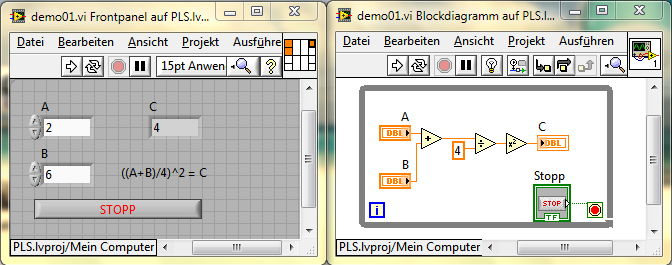
\includegraphics[width=0.7\textwidth]{Pics/demo01.png}
	\caption{VI Demonstration: Links Frontpanel, Rechts Blockdiagramm}
	\label{fig:demo01}
	\end{figure}

	%\subsection{Objektorientiertes Design}  %2-15
	\subsection{Entwurfsmuster - Design Pattern}
	\label{chap:entwurfsmuster}
Zur Entwicklung einer umfangreichen Applikation ist es unerlässlich mit Entwurfsmustern zu arbeiten. Sie helfen nicht nur dem Entwickler den Überblick nicht zu verlieren sondern machen es auch für Außenstehende einfacher den Code zu lesen und modifizieren.

LabVIEW bietet neun verschiedene Entwurfsmuster. Für welches man sich entscheidet hängt von folgenden Kriterien ab:
\begin{itemize}
	\item Gibt es eine feste Reihenfolge / Sequenzen von Befehlen?
	\item Muss das Programm mit einem User-Interface agieren?
	\item Ist die Datenverarbeitung intensiv? 
	\item Gibt es parallele Operationen?
\end{itemize}

Im folgenden gehe ich auf einige Entwurfsmuster ein, die für meine Problemstellung infrage kommen könnten. Das sind: der Zustandsautomat, Master/Slave-Entwurfsmuster, Ereignisbehandler für Benutzeroberfläche und das Erzeuger/Verbraucher-Entwurfsmuster. Später im Abschnitt \ref{chap:designpattern} werde ich auf meine Wahl des Entwurfsmuster eingehen.

\subsubsection{Zustandsautomat}%4-6
Mit jedem Zustand wird ein bestimmter Blockdiagramm Ausschnitt ausgeführt und ermittelt, zu welchem Zustand weitergesprungen wird. In einer While-Schleife wird eine Case-Struktur ausgeführt. 
%Die Case-Struktur bekommt Initialisierungs-Zustand. In jedem Case der Case-Struktur wird auf eine anderen Case oder den eigenen weiter gesprungen bis die While-Schleife ihre Abbruchbedingung erreicht hat.
	
\subsubsection{Master/Slave-Entwurfsmuster}
Bei diesem Entwurfsmuster gibt es eine Master-Schleife und mindestens eine Slave-Schleife. Die Master Schleife wird immer ausgeführt. Sie benachrichtigt Slave-Schleifen, einen bestimmten Code auszuführen. Die Slave-Schleifen werden vollständig ausgeführt und warten dann auf die nächste Benachrichtigung.

\subsubsection{Einfacher Ereignisbehandler für Benutzeroberfläche}
Dieses Entwurfsmuster wird verwendet für die Verarbeitung von Ereignissen der Benutzeroberfläche. Die Vorlage eignet sich für Dialogfelder und andere Programmoberflächen. Des Weiteren kann man benutzerdefinierte Ereignisse erzeugen und ausführen, die wie Ereignisse der Benutzeroberfläche behandelt werden.

\subsubsection{Erzeuger/Verbraucher-Entwurfsmuster} %4-10 
Hier werden zwei separate While-Schleifen unabhängig voneinander ausgeführt: Die erste Schleife erzeugt Daten, während die zweite Schleife die Daten verarbeitet. Obwohl sie parallel ausgeführt werden, werden zwischen den Schleifen über Queues Daten ausgetauscht.
Diese Vorlage bietet die Möglichkeit bei Benutzereingriffen asynchron Code auszuführen, ohne die Reaktionszeit der Benutzeroberfläche zu beeinträchtigen. 
So kann man durch die parallele Ausführung der Schleifen Leistungssteigerung des Programms erzielen. 

		
		%\paragraph{Event Handling}
		%\paragraph{Error Handling} %4-47
		
\section{Programm Analyse}
		%\subsection{Programmablaufplan} %2-18
\subsection{Daten Abstraktion}
Um in LabVIEW auf Objekten zu arbeiten gibt es Module. Das sind VIs die als Methoden agieren, sie haben Eingänge und Rückgabewerte.
\subsubsection{Objekte}
Folgende Objekte werden in der Party-Licht-Steuerung unterschieden:
\begin{description}
\item[Lichtkanal]Eine Lampe mit einer Farbe, Intensität und Nummer.
\item[Lichterset]Ein 2D-Array aus Lampen mit einer Warte-, Überblendungs- und Nachlaufzeit sowie einem Namen.
\item[Lichterset Queue] Eine Liste mit allen Lichtersets.

\item[Verbraucher Queue]Die Warteschlange für die Verbraucherschleife, hier stehen Befehle von der Erzeugerschleife drin. 

%Das Objekt besteht aus einem Cluster mit: ein "`Kommando"' vom Typ "`Enum"' und einem "`Daten"' vom Typ Variant.

%Der Datentyp "`Variant"' ist ein allgemeiner Container für alle anderen Datentypen in LabVIEW. Sind Daten in ein Variantwert konvertiert, werden die Daten und der ursprüngliche Datentyp gespeichert. So kann LabVIEW die Variantdaten zu einen anderen Zeitpunkt wieder fehlerfrei in den ursprünglichen Datentyp umwandeln. \ref{LabViewHilfe}

\item[Display Queue]Die Warteschlange für die Displayschleife, über diese kommunziert die Verbraucherschleife mit ihr. Enthält das selbe Cluster wie die Verbraucher Queue

\end{description}


\subsubsection{Module}
Dieser Abschnitt beschreibt die Module und nennt ihre Funktionen:
\begin{description}
\item[Lichterset Modul]
Das Lichterset Modul initialisiert das Lichterset Array und führt folgende Anweisungen darauf aus:
	\begin{itemize}
	\item Add Get und Set Lichterset
	\item getAnzahlLichtersets
	\item getLeeresLichterset
	\end{itemize}
%Ist eine FGV. Das Lichterset Modul initalisiert ein 1D-Array aus Lichterset Objekten(Lichterset Queue) und führt die Anweisungen Add Get und Set sowie getAnzahl und getLeeresLichterset darauf aus.

\item[Display Modul]
Dieses Modul sorgt für die Aktualisierungen auf dem Front Panel.
	\begin{itemize}
	\item Init und Update Front Panel
	\item Auswahl Lichterset aus der Lichterset-Queue
	\item De-/Aktivieren von Schaltflächen
	\item Update  Lichterset-Queue
	\end{itemize}

\item[Timing Modul] Es sorgt für die Berechnung der verschiedenen Zeiten:
	\begin{itemize}
	\item Wartezeit
	\item Überblendungszeit
	\item Nachlaufzeit
	\end{itemize}
\item[Fehler Modul] Hier wird die Fehlerbehandlung durchgeführt.
	\begin{itemize}
	\item Fehler ausgeben
	\item Fehler behandeln
	\end{itemize}

\item[Datei Modul] Das Modul sorgt für den Datei Ein- und Ausgabe.
	\begin{itemize}
	\item Speicher Lichtersets
	\item Lade Lichtersets
	\end{itemize}

\end{description}

Auf die Implementierung der Module wird im Kapitel \ref{chap:impl} eingegangen.

\subsection{Ablaufdiagramm }
Mit Ablaufdiagrammen wird der Programmfluss illustriert. Mit deren Hilfe kann man eine Aufgabe in handhabbare Funktionen teilen. Abbildung \ref{fig:plan01} zeigt das Ablauf Diagramm für die Abspiel-Funktion in der Party-Licht-Steuerung. Ein Knoten repräsentiert einen Zustand.
	\begin{figure}[!ht]
	\centering
		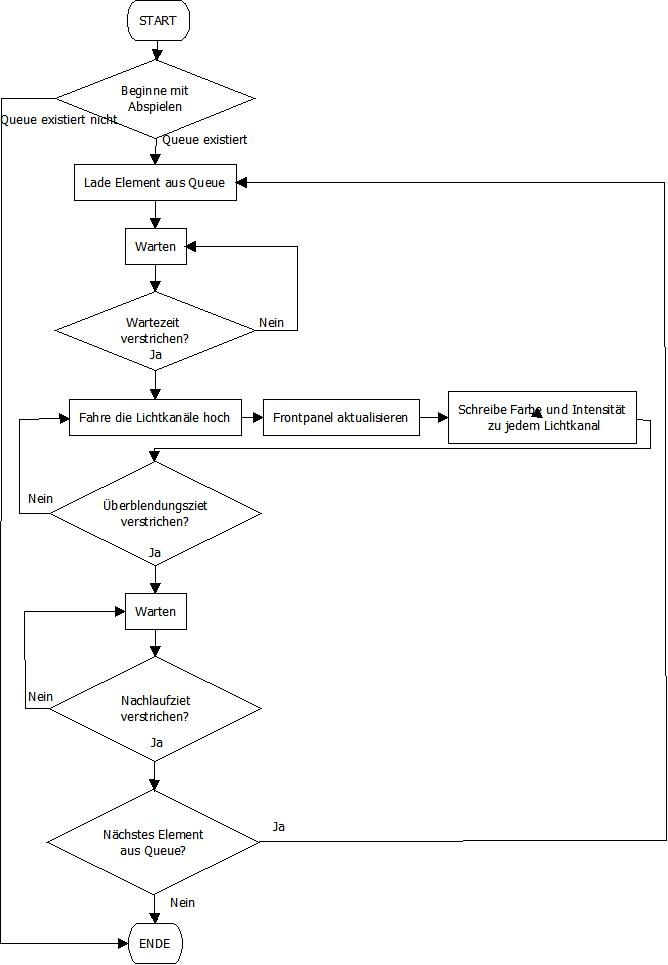
\includegraphics[height=0.9\textheight]{Pics/play-flowchart.jpeg}
	\caption{Ablaufdiagramm für die Abspiel-Funktion}
	\label{fig:plan01}
	\end{figure}	
		
\subsection{Datenfluss Diagramm}
Datenfluss Diagramme haben die Aufgabe zu zeigen, welchen Weg die Daten durch eine Applikation nehmen. Abbildung \ref{fig:plan02} zeigt das Datenfluss Diagramm für die Abspiel-Funktion in der Party-Licht-Steuerung. Die Knoten (Kreise) repräsentieren die Prozesse. Eine externe Entität ist das Licht Kontroll-System. Die Pfeile zeigen die Richtung des Datenflusses an.
	\begin{figure}[!ht]
	\centering
		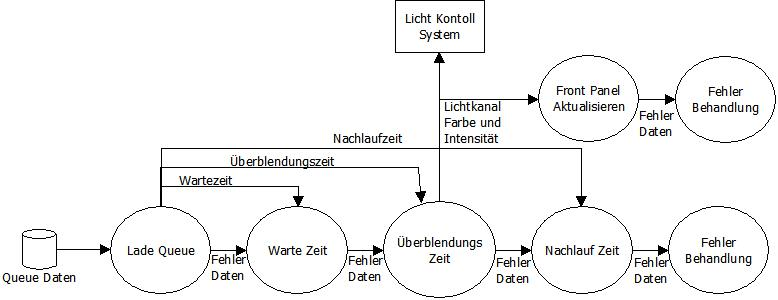
\includegraphics[width=\textwidth]{Pics/play-dataflow.jpeg}
	\caption{Datenfluss Diagramm für die Abspiel-Funktion}
	\label{fig:plan02}
	\end{figure}	

	
%\section{User Interface}

\section{Code Implementierung}
\label{chap:impl}
		\subsection{Auswahl des Design Pattern} %6-3
		\label{chap:designpattern}
		%4-18
		Bei der Wahl des Entwurfsmusters habe ich mich für das Erzeuger/Verbraucher Design  (siehe Abschnitt \ref{chap:entwurfsmuster}) entschieden. Bei diesem Pattern kann man die Ereignisbehandlung vom User-Interface und den auszuführenden Code gut trennen. 

Das Entwurfsmuster wird wie folgend abgewandelt implementiert.  Die Erzeuger Schleife reagiert auf Events vom User-Interface. Diese sind die drei Schaltflächen: Abspielen, Aufnehmen und Stoppen sowie die Menüauswahl: Speichern, Laden und Beenden.

Über eine Verbraucher-Queue tauscht die Erzeugerschleife Kommandos und Daten mit der Verbraucherschleife aus. Hier sind folgende Kommandos implementiert:
\begin{itemize}
\item initialisieren
\item aufnehmen
\item abspielen
\item stoppen
\item laden
\item speichern und
\item beenden
\end{itemize}
Daten die die Erzeuger- an die Verbraucherschleife sendet sind Lampen-Sets die beim aufnehmen, speichern oder laden entstehen. In der Verbraucherschleife werden alle Berechnungen durchgeführt. Diese Schleife kommuniziert über eine Display-Queue mit der Displayschleife.

Sie hat die Aufgabe Änderungen am User-Interface durchzuführen. Diese können sein:
\begin{itemize}
\item Initialisierung des Front Panels
\item Update der Lichtkanäle
\item Auswahl eines Lichtsets
\item De-/Aktivieren von Schaltflächen
\item Update der Set-Ablaufliste und
\item Stopp
\end{itemize}

Abbildung \ref{fig:schleifen} zeigt die Struktur aus dem Blockdiagramm. 
Die Funktionen der Applikation sind in drei separate Schleifen aufgeteilt, der Vorteil dieser Architektur ist, das die Funktionalität der einzelnen Prozesse parallel ausgeführt werden kann. Des Weiteren ist diese Art der Architektur wartungsfreundlicher und besser skalierbar. 

%Auf die Implementierung der einzelnen Funktionen wird in den folgenden Abschnitten eingegangen.

	\begin{figure}%[!ht]
	\centering
		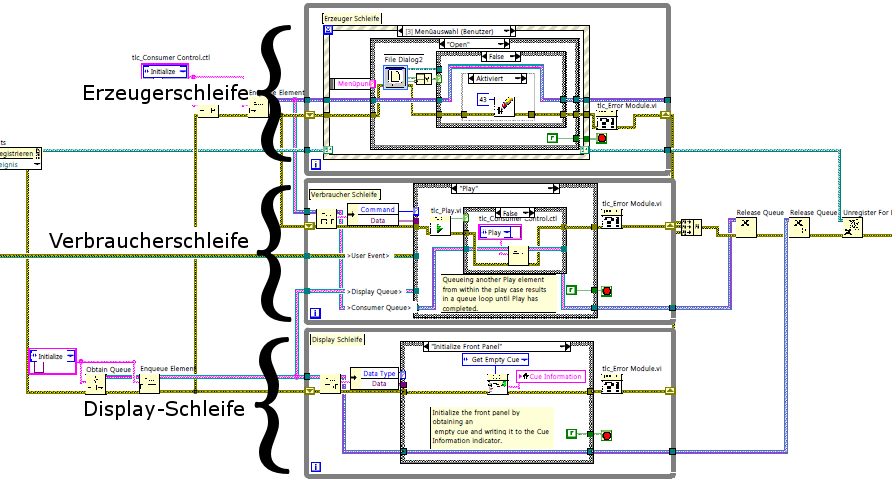
\includegraphics[width=0.9\textwidth]{Pics/ueberblick003.png}
	\caption{Design Struktur für das Blockdiagramm}
	\label{fig:schleifen}
	\end{figure}
 		

		
		
		%\subsection{Timing}
		%\subsection{Auswahl der Datentypen}

\subsection{Init und Shutdown Funktion}	%E 7-1
Die Initialisierungsfunktion wird beim Start der Anwendung ausgeführt. Die setzt alle Module in einen definierten, sicheren Zustand und säubert das User-Interface. Abbildung \ref{fig:a1} im Anhang zeigt das Blockdiagramm vom \textit{"`init.vi"'}.

Wenn der Benutzer im Menü auf Datei$\rightarrow$Beenden klickt wird die Anwendung sicher heruntergefahren, dass heißt es werden alle Speicher-Referenzen freigegeben. Abbildung \ref{fig:a2} im Anhang zeigt das Blockdiagramm vom \textit{"`shutdown.vi"'}.

\subsection{User Interface}
Die Display-Schleife sorgt für Updates auf dem User Interface.  Abbildung \ref{fig:disp} zeigt diese mit dem Stopp Case. Zu beginn wird ein Element aus der Display Queue genommen und dann nach Typ und Daten aufgeschlüsselt. Anhand des Datentyps, das die sie von der Verbraucherschleife erhalten wird der entsprechende Case aufgerufen. Bei dem Kommando Stopp wird die While-Schleife beendet. Sollte ein Fehler in einem Case aufgetreten sein, wird es vom \textit{"`Error Module.vi"'} behandelt. Dazu später mehr, im Abschnitt \ref{chap:fehler} Fehlerbehandlung. Im folgenden werden die einzelnen Cases in der Display-Schleife erläutert.

	\begin{figure}[h!]
	\centering
		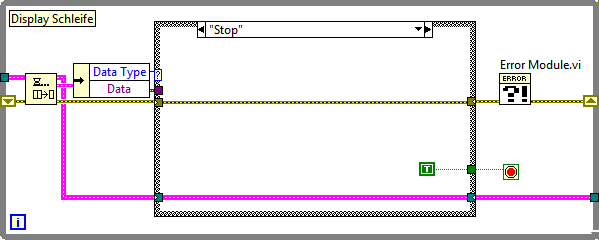
\includegraphics[width=\textwidth]{Pics/front-stop.png}
	\caption{Display Schleife}
	\label{fig:disp}
	\end{figure}

%Sie hat hat eine Case-Struktur mit den folgenden Funktionen.

\subsubsection{Initialisierung des Front Panels}
Dieser Case erstellt ein 2D-Array von Lichtkanälen und stellt es auf dem Front Panel dar. Jeder Kanal bekommt eine Nummer. Die Farbe wird auf schwarz und die Intensität auf 0 gesetzt. 

Der entsprechende Ausschnitt aus dem Programmcode ist im Anhang auf Abbildung \ref{fig:a3}.

\subsubsection{Auswahl eines Lichtsets aus der Lichterset Queue}
In diesem Case wird eine Spalte in Ablaufkontrolle hervorgehoben. Entweder wenn der User darauf klickt oder wenn die Applikation beim Abspielen über die Queue von Lichtersets iteriert. 

Der entsprechende Ausschnitt aus dem Programmcode ist im Anhang auf Abbildung \ref{fig:a4}.
 
\subsubsection{De-/Aktivieren von Schaltflächen}
Wenn eine Lichterset Queue abgespielt wird, schaltet dieser Case die Schaltfläche Aufnehmen und die Ablaufkontrollliste inaktiv. Das verhindert, das der Nutzer während eines Abspielvorgangs ein neues Lichterset anlegt oder die Ablaufkontrollliste durcheinander bringt.

Der entsprechende Ausschnitt aus dem Programmcode ist im Anhang auf Abbildung \ref{fig:a5}.

\subsubsection{Update der Set-Ablaufliste}
Dieser Case aktualisiert die Liste in der Ablaufkontrolle immer wenn ein neues Lichterset aufgenommen wurde.

Der entsprechende Ausschnitt aus dem Programmcode ist im Anhang auf Abbildung \ref{fig:a6}.

\subsubsection{Update der Lichtkanäle}
Dieser Case updatet das 2D-Array aus Lichtkanälen. Es wird immer dann aufgerufen, wenn sich Lichtkanal Daten ändern. Das ist der Fall wenn eine Lichterset Queue abgespielt wird und sich die Farbe und Intensität der Kanäle ändert oder der Nutzer auf ein Element in der Ablaufkontolle klickt um sich Informationen zum ausgewählten Lichterset anzuzeigen.

Der entsprechende Ausschnitt aus dem Programmcode ist im Anhang auf Abbildung \ref{fig:a7}.


\subsection{Aufnahme-Funktion}	
Klickt der Anwender auf die Aufnahme Schaltfläche öffnet sich eine Dialogbox in der er nach Parametern für das zu erstellende Lichterset gefragt wird. Die einzugebenden Werte sind:
\begin{itemize}
\item Setname
\item Wartezeit
\item Überblendungszeit
\item Nachlaufzeit und
\item Einstellungen für die einzelnen Lichtkanäle
\end{itemize}

Nach Bestätigung über die OK-Schaltfläche werden die gesammelten Daten in die Queue geschrieben und das User-Interface geupdated. 

Die Abbildung \ref{fig:rec} zeigt die Erzeuger-(oben) und Verbraucherschleife(unten). In der Erzeugerschleife wird die Dialogbox geöffnet. Sie gibt ein Objekt mit den gesammelten Daten zurück. Wurde der Dialog nicht abgebrochen werden die Daten zusammen mit dem Kommando "`record"' in die Verbraucher Queue gesteckt. Die Verbraucherschleife nimmt sich das Objekt aus der Queue und hängt das neue Objekt an die Lichterset-Liste an. Dann gibt sie das Kommando zum updaten des User-Interface an die Display-Schleife.

	\begin{figure}[!ht]
	\centering
		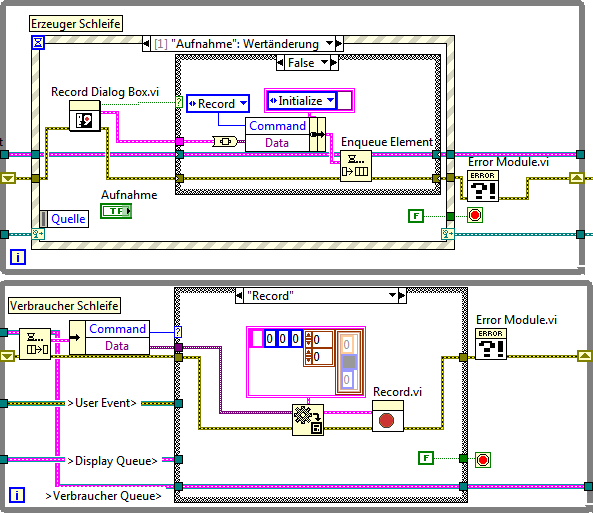
\includegraphics[width=\textwidth]{Pics/record.png}
	\caption{Aufnahme-Funktion}
	\label{fig:rec}
	\end{figure}
	
	
\subsection{Timing}
Zur akkuraten Berechnung der Warte-, Überblendungs- und Nachlaufzeit beim Abspielen der Lichtersets dient das Timing VI. Dieses VI arbeitet als funktionale globale Variable (FGV).

\subsubsection{Funktional globale Variable}
In funktionalen globalen Variablen (FGVs) können in nicht initialisierten Schieberegistern von While- oder For-Schleifen Daten gehalten werden. 
Die Daten bleiben erhalten, solange sich das zugehörige VI im Speicher befindet. Die jeweilige Schleife in einer FGV wird bei einem Aufruf nur einmal durchlaufen. Liegen die Daten am Ende der Schleife (rechts) im Schieberegister an, stehen diese beim nächsten Aufruf wieder am Anfang (links) an. Das hat den Vorteile das Daten nicht immer bei jedem VI Aufruf mit geführt werden müssen. Die Daten werden einmal beim initialisieren mitgegeben halten sich dann im Speicher. \cite{LabViewHilfe}

Die Timing FGV hat zwei Kommandos: starten bzw. initialisieren und checken. Die Auswahl wird über eine Switch-Case-Anweisung getroffen. Soll eine Zeit gemessen werden, wird zu beginn der Messung das Timing VI mit der Ziel-Zeit und dem Kommando Start aufgerufen. Hier wird die aktuelle Systemzeit in Sekunden ermittelt (Startzeit) und ins Schieberegister geschrieben. In der Applikation wird in einer Schleife dann immer mit dem Kommando check abgefragt ob die Zeit abgelaufen ist. Ist das der Fall, gibt die FGV am Ausgang "`Verstrichen"' True zurück, sonst False. Abbildung \ref{fig:timing} zeigt die FGV mit ihren beiden Cases. 

	\begin{figure}[h!]
	\centering
		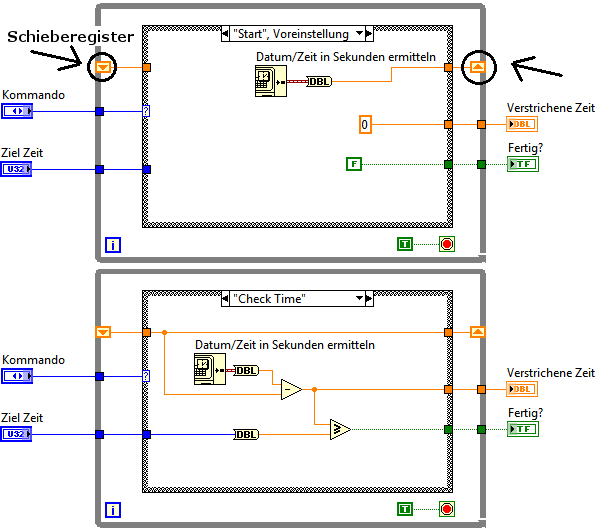
\includegraphics[width=\textwidth]{Pics/timing.png}
	\caption{FGV Timing VI}
	\label{fig:timing}
	\end{figure}


\subsection{Abspiel-Funktion}
Die Abspiel-Funktion wird als Zustandsautomat implementiert. Das Flussdiagramm aus Abbildung \ref{fig:plan01} zeigt die einzelnen Zustände. 

Empfängt die Verbraucherschleife das Kommando zum Abspielen öffnet sie das \textit{"`record.vi"'}. Das VI durchläuft ein Zustand. Gibt es zurück, das der Zustandsautomat noch nicht bis zum Ende durchgelaufen ist, steckt die Verbraucherschleife erneut das Kommando play in die Verbraucher Queue. Daraus resultiert eine Schleife in der bei jeder iteration ein Zustand durchläuft, solange bis der Zustandsautomat am Ende ist.
Zur Berechnung, ob die verschieden Zeiten abgelaufen sind wird das  \textit{"`timing.vi"'} aufgerufen. Im Anhang in Abbildung \ref{fig:a9} findet sich der Code für den Zustand Überblenden.

\subsection{Stopp-Funktion}
Will der Bediener den Abspiel-Vorgang abbrechen, klickt er auf die Stopp Schaltfläche. Jetzt wird der Zustandsautomaten der Abspiel-Funktion unterbrochen. Das geschieht indem die Verbraucher Queue geleert und der Zustandsautomat zurückgesetzt wird. So wird garantiert, das keine Nachrichten mehr in der Verbraucher-Queue sind und der Zustandsautomat beim nächsten Anlauf wieder am Anfang startet. Der Code kann im Anhang bei Abbildung \ref{fig:a10} gefunden werden.
		
		
\subsection{Speichern und Lade Funktion}
Die Funktionalität zum speichern und laden in eine Datei ist für ein LJ unerlässlich. So kann er während einer Probe alle Einstellungen setzen und diese in eine Datei schreiben. Zum Zeitpunkt des Events muss die Datei nur noch geladen werden. 

Zum speichern oder laden klickt der LJ in die Menüleiste unter Datei auf speichern bzw. laden. Die Applikation (Erzeugerschleife) öffnet ein File-Dialog und prüft ob die ausgewählte Datei existiert. Dann schickt sie das entsprechende Kommando (load oder save) zusammen mit dem Dateipfad an die Verbraucherschleife.

\subsubsection{In Datei speichern}
In der Verbraucherschleife wird über eine For-Schleife ein 1D-Array aus Lichtersets erstellt. Dieses wird an das \textit{"`File-Modul.vi"'} übergeben. Hier wird das 1D-Array in die angegebene Datei geschrieben. Hierfür die vorgefertigten LabView VIs genutzt: Öffnen, Schreiben und Schließen einer Datei. Der Code ist im Anhang unter Abbildung \ref{fig:a11}.

\subsubsection{Aus Datei laden}
Um aus einer Datei Elemente lesen zu können muss man der Lese-Funktion den Lichterset Datentyp mitgeben. Zurück bekommt man ein 1D-Array aus Lichtersets. Diese wird dann in die Lichterset Queue geschrieben. Der Code ist im Anhang unter Abbildung \ref{fig:a12}.


\subsection{Fehlerbehandlung}
\label{chap:fehler}
Zur Fehlerbehandlung gehört das sichere herunterfahren der Applikation wenn ein Fehler auftritt. Um die Erzeugerschleife zu beenden muss ein User-Event erzeugt werden. Die Verbraucherschleife wird beendet in dem das Kommando Exit in die Verbraucher Queue geschrieben wird. Zum beenden der Display-Schleife wird das Kommando Stopp an die Display Queue gesendet. Empfängt eine Schleife solch ein Kommando bzw. Event wird die Abbruchbedingung auf true gesetzt. Sind alle drei Schleifen beendet, wird in der letzten Sequenz der Applikation die Verbraucher und Display Queue freigegeben, die Ereignisregistrierung aufgehoben, die Benutzerereignisse gelöscht, der aufgetretene Fehler ausgegeben und die LabVIEW Anwendung beendet.

Der Code, der im Fall eines oder mehrere Fehler ausgeführt wird ist im Anhang unter Abbildung \ref{fig:a13} zu finden.


\section{Stress und Lade Test}		
Bevor die Anwendung freigegeben wird ist es notwendig die Leistung und Handhabbarkeit der Applikation zu testen. 

Für den Test der Party-Licht-Steuerung wird ein VI geschrieben das 10.000 Lichtersets mit zufälligen Parametern für die Warte-, Überblendungs- und Nachlaufzeit sowie Lichtfarbe und -intensität in eine Datei schreibt. 

Als Testwerkzeug dient der Windows Task-Manager. Er läuft mit während die Testdatei in die Anwendung geladen und abgespielt wird. Mit Hilfe des Windows Task-Manager kann überprüft werden, ob während der Laufzeit ein Leistungs- oder Speicherfehler auftritt. 

Die Anwendung wurde auf einem Notebook mit einem Intel Core2 Duo Prozessor (2,17GHz) und 2 GB Hauptspeicher ausgeführt. 

Abbildung \ref{fig:test} zeigt den Verlauf der Prozessor- und Arbeitsspeicher Auslastung während des Tests. Das erste rot umrahmte Viereck (von links nach rechts) zeigt den Ladevorgang der Applikation. Es werden circa 40 MB in den Arbeitsspeicher geladen. Das zweite Viereck umrahmt das laden der Testdatei (2,7 MB) hierfür werden in Arbeitsspeicher ungefähr 102 MB reserviert. Damit beansprucht die gesamte Applikation 141 MB des Hauptspeichers. Das letzte Viereck zeigt  den Abspielvorgang bis zum 140. Lichterset. Nach ungefähr 4 Stunden sind alle 10.000 Sets durchgelaufen danach konnte die Anwendung ohne Fehler beendet werden und der zuvor reservierte Speicher wieder freigegeben. Während des Abspielvorgangs war der Prozessor im Mittel mit 14\% ausgelastet.

Aus dem Test lässt sich das Ergebnis ziehen, das kein Speicherüberlauf auftrat, kein Speicher unnötig allokiert wurde und der Prozessor mit der Anwendung nicht überlastet war. Somit gilt der Test als bestanden. 

	\begin{figure}%[]
	\centering
		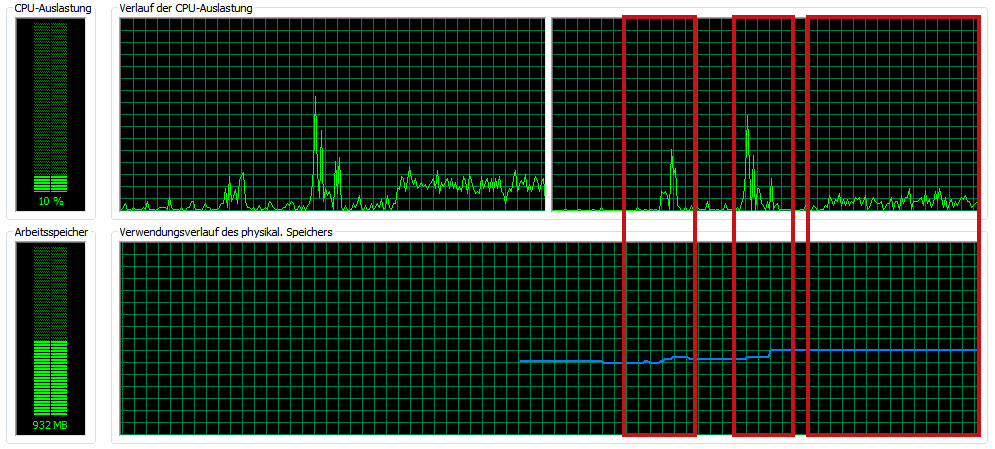
\includegraphics[width=\textwidth]{Pics/test04.png}
	\caption{Verlauf der Prozessor- und Arbeitsspeicher Auslastung}
	\label{fig:test}
	\end{figure}


\section{Einsetzen der Anwendung}
LabVIEW bietet die Möglichkeit über ein Dialog aus einem Projekt heraus eine ausführbare Windows- (.exe) oder MAC OS (.app) Anwendung oder Installer zu erstellen. 
Eine ausführbare Windowsanwendung und ein Installer mit der notwendigen Laufzeit-Umgebung finden sich auf der beigefügten CD. Für die Laufzeit-Umgebung gibt es eine kostenfreie Lizenz, sie kann beliebig oft vervielfältigt werden.

Die Mindestvoraussetzungen für ein Windowssystem sind \cite{ni-min}: 
\begin{itemize}
\item Prozessor: Pentium III/Celeron 866 MHz oder gleichwertig
\item Hauptspeicher: 256 MB
\item Festplattenspeicher: 1 GB
\item Betriebssystem: XP
\end{itemize}
%http://www.ni.com/labview/requirements/d/

\subsection{Webservice}
Mit LabVIEW lässt sich ein Webinterface erstellen auf das der Anwender via Inter- oder Intranet mit einem Standartbrowser zugreifen kann. Rechenintensive Anwendungen können von einer Serverfarm bearbeitet werden und müssen nicht die Rechnerressourcen des Hosts beanspruchen. Auch lassen sich mit einem Webservice, Prozesse von der Ferne aus überwachen. Anwendungen hierfür wären zum Beispiel die Produktionsüberwachung für die Produktionsleitung. Mitarbeiter müssten nicht mehr von Maschinenterminal zu Maschinenterminal laufen sondern könnten zum Beispiel von einem Heimarbeitsplatz die ganze Produktionsanlage überwachen.



\section{Abschließende Betrachtung}
Bei dem Projekt ist eine voll funktionsfähige LabVIEW Anwendung entstanden, somit konnte das Projekt erfolgreich abgeschlossen werden. 

\subsection{Fazit}
Ein wichtiger Vorteil in der graphischen Programmierung von LabVIEW ist die Einfachheit parallele Abläufe zu programmieren. So reicht es aus zwei Sub-VIs ohne Datenabhängigkeit nebeneinander zulegen. Man muss jedoch auf mögliche "`Race Conditions"' achten, hierfür stehen verschiedene Möglichkeiten zur Verfügung. Zum Beispiel Semaphore oder Warteschlangen. 

Das Front Panel von LabVIEW hat gezeigt, das es ein bequeme Möglichkeit bietet, schnell und gute Bedienoberflächen zu erstellen.

Im Blockdiagramm ist durch die graphische Darstellung des Programmablaufs die Lesbarkeit deutlich einfacher. Anhand verschiedener Farben lassen sich die Datentypen und ihr Ursprung besser erkennen.

Ein weiteren Vorteil den LabVIEW bietet ist die Unterstützung von Kommunikationsprotokollen wie TCP/IP. Es ist somit möglich auch weit entfernte Anwendungen zu steuern und nutzen.

Bei der Entwicklung von LabVIEW Programmen gibt es auch Nachteile, so ist man an die originale LabVIEW-Entwicklungsumgebung von National Instruments gebunden. Für diese fallen Lizenzen an. Die "`NI Developer Suite Core"' für Windows kostet 5.800 Euro, hier gibt es auch kostenlose Versionen mit verminderten Funktionsumfang für Studenten. \cite{ni-kost}
%http://ohm.ni.com/advisors/devsuite/pages/cds/newcustomer.xhtml

Auf einen weiteren Nachteil stößt man, wenn man LabVIEW-Programme verteilen will. Hat das Zielsystem keine Entwicklungsumgebung, ist es nötig eine Laufzeitumgebung zu installieren. Diese ist für die meisten Module kostenfrei.

Auch bei strukturierter Programmierung können kleine Änderungen im Programmfluss   aufwendige Neustrukturierungen nach sich ziehen. Ärgerlich ist es beim Schaffen vom Raum im Blockdiagramm immer wieder Drähte und Symbole neu ordnen zu müssen.

	
%	\subsection{Update }%E8-2
%	\subsection{Information Hiding} %E4-5
	
\subsection{Ausblick auf Erweiterungen}
Die Party-Licht-Steuerung bietet noch Möglichkeiten für Erweiterungen.

\subsubsection{Ansteuerung von Hardware}
Möchte man externe Lichtkanäle ansteuern könnte man ein dritte Verbraucher Schleife hinzufügen. Diese muss dann einen "`Data Acquisition-Task"' starten und die Ausgänge setzen. Als anzusteuernde Hardware empfiehlt sich das NI PCI-6723 Analogausgangsmodul. Es hat 32 Analogausgänge, damit könnte man von 16 Lampen die Farbe und Intensität steuern.\cite{ni-pci}

	\begin{figure}[h!]
	\centering
		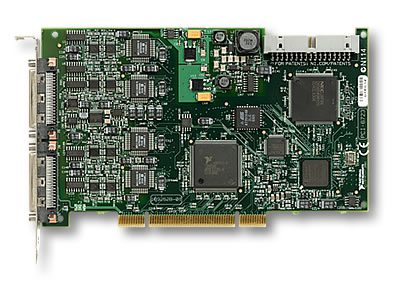
\includegraphics[width=0.5\textwidth]{Pics/pci6723.jpg}
	\caption{NI PCI-6723 mit 32 Analogausgänge \cite{ni-pci} }
	\label{fig:a7}
	\end{figure}

%http://sine.ni.com/nips/cds/view/p/lang/de/nid/12551



\subsubsection{Multilingualität}
Um die Applikation einer größeren Masse an Anwendern zur Verfügung zu stellen konnte eine Mehrsprachigkeit implementiert werden. Dazu könnte beim Start der Anwendung der Nutzer nach seiner Sprache gefragt werden. Über eine Tabelle mit der zur Verfügung stehenden Sprachen könnte ein Auswahl für die Beschriftung der Front Panel Elemente getroffen werden.

	
%	\subsection{Probleme}


